\tikzset{every picture/.style={line width=0.75pt}} %set default line width to 0.75pt        

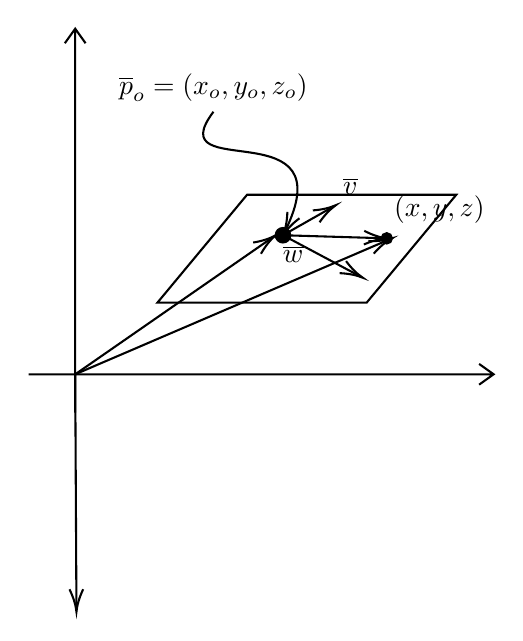
\begin{tikzpicture}[x=0.75pt,y=0.75pt,yscale=-1,xscale=1]
%uncomment if require: \path (0,435); %set diagram left start at 0, and has height of 435

%Shape: Axis 2D [id:dp7235801239941206] 
\draw  (180,181.5) -- (404,181.5)(202.4,15) -- (202.4,200) (397,176.5) -- (404,181.5) -- (397,186.5) (197.4,22) -- (202.4,15) -- (207.4,22)  ;
%Shape: Boxed Line [id:dp007075143317909038] 
\draw    (202.4,181.5) -- (202.99,294) ;
\draw [shift={(203,296)}, rotate = 269.7] [color={rgb, 255:red, 0; green, 0; blue, 0 }  ][line width=0.75]    (10.93,-3.29) .. controls (6.95,-1.4) and (3.31,-0.3) .. (0,0) .. controls (3.31,0.3) and (6.95,1.4) .. (10.93,3.29)   ;
%Shape: Parallelogram [id:dp6034958675104498] 
\draw   (285.2,95) -- (386,95) -- (342.8,147) -- (242,147) -- cycle ;
%Shape: Circle [id:dp8192565860314898] 
\draw  [fill={rgb, 255:red, 0; green, 0; blue, 0 }  ,fill opacity=1 ] (299,114.5) .. controls (299,112.57) and (300.57,111) .. (302.5,111) .. controls (304.43,111) and (306,112.57) .. (306,114.5) .. controls (306,116.43) and (304.43,118) .. (302.5,118) .. controls (300.57,118) and (299,116.43) .. (299,114.5) -- cycle ;
%Curve Lines [id:da8374672565974479] 
\draw    (269,55) .. controls (242.14,90.82) and (334.07,52.39) .. (302.98,113.57) ;
\draw [shift={(302.5,114.5)}, rotate = 297.47] [color={rgb, 255:red, 0; green, 0; blue, 0 }  ][line width=0.75]    (10.93,-3.29) .. controls (6.95,-1.4) and (3.31,-0.3) .. (0,0) .. controls (3.31,0.3) and (6.95,1.4) .. (10.93,3.29)   ;
%Straight Lines [id:da7811790552449687] 
\draw    (302.5,114.5) -- (339.23,134.06) ;
\draw [shift={(341,135)}, rotate = 208.03] [color={rgb, 255:red, 0; green, 0; blue, 0 }  ][line width=0.75]    (10.93,-3.29) .. controls (6.95,-1.4) and (3.31,-0.3) .. (0,0) .. controls (3.31,0.3) and (6.95,1.4) .. (10.93,3.29)   ;
%Straight Lines [id:da2105628435048088] 
\draw    (302.5,114.5) -- (350.5,115.94) ;
\draw [shift={(352.5,116)}, rotate = 181.72] [color={rgb, 255:red, 0; green, 0; blue, 0 }  ][line width=0.75]    (10.93,-3.29) .. controls (6.95,-1.4) and (3.31,-0.3) .. (0,0) .. controls (3.31,0.3) and (6.95,1.4) .. (10.93,3.29)   ;
%Shape: Circle [id:dp9717418239463027] 
\draw  [fill={rgb, 255:red, 0; green, 0; blue, 0 }  ,fill opacity=1 ] (350,116) .. controls (350,114.62) and (351.12,113.5) .. (352.5,113.5) .. controls (353.88,113.5) and (355,114.62) .. (355,116) .. controls (355,117.38) and (353.88,118.5) .. (352.5,118.5) .. controls (351.12,118.5) and (350,117.38) .. (350,116) -- cycle ;
%Straight Lines [id:da6864844735404465] 
\draw    (202.4,181.5) -- (297.36,115.64) ;
\draw [shift={(299,114.5)}, rotate = 145.26] [color={rgb, 255:red, 0; green, 0; blue, 0 }  ][line width=0.75]    (10.93,-3.29) .. controls (6.95,-1.4) and (3.31,-0.3) .. (0,0) .. controls (3.31,0.3) and (6.95,1.4) .. (10.93,3.29)   ;
%Straight Lines [id:da9050556579363687] 
\draw    (202.4,181.5) -- (353.16,116.79) ;
\draw [shift={(355,116)}, rotate = 156.77] [color={rgb, 255:red, 0; green, 0; blue, 0 }  ][line width=0.75]    (10.93,-3.29) .. controls (6.95,-1.4) and (3.31,-0.3) .. (0,0) .. controls (3.31,0.3) and (6.95,1.4) .. (10.93,3.29)   ;
%Straight Lines [id:da5591626096296052] 
\draw    (302.5,114.5) -- (326.26,100.99) ;
\draw [shift={(328,100)}, rotate = 150.38] [color={rgb, 255:red, 0; green, 0; blue, 0 }  ][line width=0.75]    (10.93,-3.29) .. controls (6.95,-1.4) and (3.31,-0.3) .. (0,0) .. controls (3.31,0.3) and (6.95,1.4) .. (10.93,3.29)   ;

% Text Node
\draw (269,51.6) node [anchor=south] [inner sep=0.75pt]    {$\overline{p}_{o} =( x_{o} ,y_{o} ,z_{o})$};
% Text Node
\draw (330,96.6) node [anchor=south west] [inner sep=0.75pt]    {$\overline{v}$};
% Text Node
\draw (354.5,110.1) node [anchor=south west] [inner sep=0.75pt]    {$( x,y,z)$};
% Text Node
\draw (301,117.9) node [anchor=north west][inner sep=0.75pt]    {$\overline{w}$};


\end{tikzpicture}
